\section{Introduction}\label{sec:intro}

Getting a quicker validation of the proposed product is crucial in the era of fierce competition and faster obsolescence. Digital product development, which includes, modeling by CAD and analysis by CAE plays a crucial role in quicker ``Time to market''.  For sheet-metal/plastic products (generically classified as `thin-walled'),  a quicker and fairly accurate CAE analysis is possible by idealizing their solid models to the equivalent surface representation called ``Midsurface''. \added[remark={Reviewer 2(1):  whether this is an important problem}]{Such idealization is extremely important as stated by a Sandia report, which says that for complex engineering models, idealized models creation amounts to about 60\% of overall analysis time, whereas the mesh generation consumes about 20\% and solving the actual problem takes about 12\% \cite{Ming2012}}. 

Midsurface can be envisaged as a surface lying midway of a thin-walled solid, and mimicking \added{its shape}.   In CAE analysis, instead of using expensive 3D elements, 2D elements are used on the midsurface for fairly accurate results in far lesser computations/time. Because of this  advantage, midsurface is widely used and is available in many commercial CAD-CAE packages.  Even in this age of scalable and near-infinite computing power, it is still desirable to \replaced{idealize}{ have  a robust and well-connected midsurface,} so as to run more design iterations quickly.  \footnote{By ``robust'', it is meant that any small change in the input model should not have dramatic effect on the output midsurface and by ``well-connected'', it is meant that the midsurface should not have any gaps or overlaps and it should mimic the input correctly, especially at the connections.}

\begin{figure}[!htp]
\centering
\includegraphics[width=0.6\linewidth]{..//Common/images/MidsurfaceErrorsMscApexHighlighted}
\caption{Midsurface \replaced[remark={Reviewer 1(3): In Figure 1, highlighting the errors pictorially might be better}]{with errors shown }{Errors} (Source: \cite{MScApex})}
\label{fig:midsurfaceerrors}
\end{figure}

In spite of its demand and popularity, the existing techniques \deleted{for computing the midsurface} fail to compute a well-connected midsurface, especially for non-trivial shapes \cite{ Robinson2006, Stolt2006, Lockett2008}. Failures manifest in the form of gaps, missing patches, overlapping surfaces, not lying midway, not mimicking the input shape, etc. (Figure \ref{fig:midsurfaceerrors}). Correcting these errors is mostly a manual, tedious and highly time-consuming task, requiring hours to days. This correction time can be nearly equivalent to the time it can take to create the midsurface manually from scratch \cite{Stolt2006}. 

One of the major impediments in the development of the algorithm for automatic computation of the midsurface, is the lack of its precise definition \cite{Ramanathan2004}.  Expectations vary based on the application context (Figure \ref{fig:introduction:midsurfaceexptations}). For applications such as CAE, Figure ~\ref{fig:introduction:stairsfl} \replaced[remark={Reviewer 1(3):  write a sentence saying why 2c is relevant for CAE}]{ shows required midsurface, where there are no sharp corners \replaced{else there will be}{which will produce} unnecessary dense meshing, where as }{may be preferred over} Figure ~\ref{fig:introduction:stairsmk} is best suited for  shape matching/retrieval. Figure ~\ref{fig:introduction:stairsseparate} may be used where a disconnect needs to be highlighted. \deleted{Figure ~\ref{fig:introduction:stairsmk} is considered as the choice of midsurface for this work.}The variations shown in Figure \ref{fig:introduction:midsurfaceexptations} pertain to the geometries computed  at the interfaces, and the proposed method can cater to them too, with additional rules (for future scope). \deleted[remark={Author:Removed for Brevity}]{For specific applications such as CAE, additional rules, such as use of symmetry, specification of continuity between patches, etc. can also be incorporated to further customize the midsurface.}

\def \myfigstairspcolumnwidth{0.2}

\begin{figure}[h!]
\centering     %%% not \center
\subfloat[Model]{\label{fig:introduction:stairsmodel}\includegraphics[width=\myfigstairspcolumnwidth\linewidth]{../Common/images/Stairs_part.pdf}} \quad
\subfloat[Gradual]{\label{fig:introduction:stairsfl}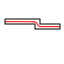
\includegraphics[width=\myfigstairspcolumnwidth\linewidth]{../Common/images/Stairs_follows.pdf}}  \quad
\subfloat[Mimicking]{\label{fig:introduction:stairsmk}
\includegraphics[width=\myfigstairspcolumnwidth\linewidth]{../Common/images/Stairs_mimic.pdf}}   \quad
\subfloat[Disjoint]{\label{fig:introduction:stairsseparate}
\includegraphics[width=\myfigstairspcolumnwidth\linewidth]{../Common/images/Stairs_separate.pdf}}
\caption{Expectations vary with regards to desired Midsurface}
\label{fig:introduction:midsurfaceexptations}
\end{figure}


The motivation of this work  is to address midsurface problems by leveraging feature-based simplification, abstraction and decomposition\deleted{in a generic manner}. \added[remark={Reviewer 2:  what is the research contribution or novelty of this work, especially the feature-based approach. }]{Although feature-based CAD modeling paradigm is prevalent for decades, many of the processes, like defeaturing, midsurface computation, etc. do not leverage it and are based on the final B-rep. Reason being, typically when these CAD models are transferred to CAE, feature information was either removed (for proprietary reasons), or neutral formats without feature supports were used, or feature-data access was not given through programming interfaces. Now, with far more integrated CAD-CAE environments, feature-information access is getting available through Application Programming Interfaces (APIs) and thus feature-based algorithms can leverage it, as demonstrated in this work}.

\added[remark={Reviewer 1: A precise description of what they mean by ``generic''. Is the generic nature of the proposed approach in terms of its scalability to a wide variety of parts?}]{Many of the earlier works were limited in the geometries they could work on (say, only planar or analytic surfaces), sub-shapes/features they could work on (say, only extruded, positive primitives), connection types they could handle (say, only, parallel, or perpendicular), etc. By proposing a `generic' methodology  here, it is implied that, in principle, no such restrictions are present in this approach. It can be made to cater to any geometry types, feature/sub-shape types or connections.} Advantages can be seen in the range of shapes handled as well as in the minimization of failures \added{(Table \ref{tbl_fbcm})}.






